% -*-coding: utf-8 -*-

V této kapitole popíšeme několik vybraných optimalizačních algoritmů. Zdaleka nejde o průřez všemi typy algoritmů\footnote{obsáhlejší přehledy lze nalézt například v \cite[p.~23]{GO ebook}, \cite{wiki metaheur}}, ale alespoň získáme představu s čím se budeme muset při hledání obecného formalismu potýkat. Na konci zmíníme obecné principy, myšlenky a problémy, které se objevují napříč všemi algoritmy, a které bychom taktéž chtěli v našem modelu pokrýt.

\section{Základní pojmy}

\par{\textbf{Účelová funkce (fitness)} je funkce, jejíž hodnotu se algoritmus snaží optimalizovat. Optimalizaci lze vždy formulovat jako minimalizaci.}

\par{\textbf{Kandidátní řešení (jedinec)} je struktura data, z nichž je možné spočíst hodnotu účelové funkce. Manipulací s těmito daty se algoritmus snaží najít nejlepší možné řešení.}

\par{\textbf{Stavový prostor} je prostor všech jedinců.}

\par{\textbf{Populace} je soubor jedinců s nimiž algoritmus aktuálně pracuje. Ne každý algoritmus potřebuje populaci}

\par{Metaheuristika je obecný návrh algoritmu popisující myšlenky, jakými budeme jedince krok po kroku zlepšovat aniž bychom dělali složitější předpoklady o účelové funkci, charakteru problému nebo implementaci. Myšlenky obsažené v metaheuristice zřídkakdy zajišťují konvergenci algoritmu k optimálnímu řešení.}

\section{Algoritmy}

\note{dát se i základní RS a Hill Climbing? ... když ano, tak citovat, nebo jsou to obecně známé věci?}

\subsection{Simulované žíhání a zrychlené simulované žíhání}

Simulované žíhání (SA -- Simulated Annealing) \cite{SA Hajek}, \cite{SA Tsitsiklis} je metaheuristika založená na analogii s chladnutím kovu. Při chladnutí se atomy snaží zaujmout pozici s co nejnižší energií; když je teplota vysoká, Brownův pohyb je intenzivní a atomy se často dostávají i do stavů s vyšší energií než měly dříve, což jim umožňuje uniknout z lokálních minim energie. Naproti tomu při nízké teplotě se atomy pohybují již téměř výhradně do stavů s nižší energií. Správnou rychlostí ochlazování (cooling schedule) Pak můžeme dosáhnout ideálně homogenního krystalu, nebo alespoň velkých zrn.

Nového jedince pomocí algoritmu SA získáme následujícím způsobem \cite[p.~1153]{SA survey}:
\begin{enumerate}
  \item $x_{new} \sim N(x_i, \sigma^2)$, $\sigma$ pevně zvolené
  \item Pokud $E(x_{new}) < E(x_i) \Rightarrow x_{i+1} \leftarrow x_{new}$,
  \item jinak $x_{i+1} \leftarrow x_{new}$ s pravděpodobností $exp(-\frac{E(x_{new}) - E(x_i)}{T_i})$,
    \newline kde $T_i = \frac{T_0}{ln(i)}$, $i$ je krok.
\end{enumerate}

\note{různé prameny uvádějí různé přístupy: např. u \cite{VFSA} je mutace i pravd. příjmu parametrizovaná teplotou -- takže je to vlastně quantum SA a důkazy konvergence nejsou vedeny přes přijímací pravd, ale přes mutaci. Na druhou stranu, důkazy v Hájkovi a Tsitsiklisovi jsou vedeny přes přijímací pravd. a předpoklady o okolí jsou poměrně volné...}

V \cite{SA Hajek}, \cite{SA Tsitsiklis} je dokázáno, že pro dostatečně vysoké $T_0$, při daném postupu ochlazování $x_i \xrightarrow{i \to +\infty} x_{opt}$ podle pravděpodobnosti. Zastavení algoritmu určujeme volbou cílové teploty (běžně i řádu $10^{-4}$) z čehož vyplývá okamžitá nevýhoda SA a tou je v praxi příliš pomalý pokles teploty.

\note{článek od Szu nemůžu sehnat.... na Esevieru jako jediný nemá pdf...}

\subsection{Genetická optimalizace \note{myslíme binary strings, nebo celé EA?}}

Genetická optimalizace se rozvíjí zhruba od 50.let, kdy vznikla jako analogie pro přírodní evoluci a do dnešní doby se rozvětvila na řadu směrů zabývajících se specifickými třídami problémů, na které je možno GO použít. Obsáhlý přehled literatury o GO lze nalézt např v \cite[p.~]{GO ebook}. Nás nyní zajímá GO hlavně jako metaheuristika. Jedná se o populační algoritmus a od SA a FSA se liší hlavně tím, že nový jedinec vzniká reprodukcí z dvou a více jedinců z minulé generace. Po počáteční inicializaci (většinou náhodná) se průběh GO dá popsat následujícím flowchartem:

\begin{figure}[h!]\label{EA fig}
  \includegraphics[width=\textwidth]{img/EA}
\end{figure}





\subsection{Diferenciální evoluce}

Diferenciální evoluce \cite{DE Storn} je optimalizační algoritmus vhodný pro mnohodimenzionální stavové prostory. Strukturou je podobný \note{předchozímu - EA, GO??}, jen reprodukce je o něco složitější:

\begin{figure}[h!]\label{DE fig}
  \includegraphics[width=\textwidth]{img/DE}
\end{figure}

\subsection{Evoluční strategie}

\section{Dílčí principy optimalizačních algoritmů}

\subsection{Globální VS lokální hledání}

Neboli diverzifikace versus intenzifikace. Jsou dvě hranice mezi nimiž se optimalizační algoritmy pohybují. Globální prohledávání se snaží co nejrovnoměrněji navzorkovat celý stavový prostor (dostat jedince v populaci co nejdále od sebe) a jeho průběh prakticky nezávisí na předchozích stavech algoritmu. Ten se tak efektivně vyhne uvíznutí v lokálním minimu, avšak nemá šanci vylepšit případné slibné jedince. Globálním prohledáváním nelze tedy dosáhnout optimální výsledku, jeho výkonnost je však zcela nezávislá na charakteru účelové funkce. Typickým příkladem čistě globální heuristiky je náhodné prohledávání.

Lokální prohledávání naopak jedince po malých krocích stále vylepšuje. Pokud již jedinec vylepšit nejde (v okolí není žádný s nižší účelovou funkcí), skončí. Chová se tedy přesně opačně než globální prohledávání -- zákonitě uvízne v každém globálním minimu, ale jedince \bq vytěží\eq na maximum. Pro jiné, než unimodální účelové funkce také nedává optimální řešení. Jeho příkladem je například Shoot\&Go (Hill-climbing).

Protože žádný z přístupů není optimální, snaží se je algoritmy vhodně staticky, nebo adaptivně kombinovat.

\subsection{Elitismus}

Tento pojem se zrodil u evolučních algoritmů a je pokusem, jak v populaci implementovat lokální prohledávání. U EA se často při přechodu do nové generace celá populace zahodí a nahradí se potomstvem, nebo jeho částí. Tím se však vzdává šance podrobněji prozkoumat okolí dobrých jedinců. Proto se při tvorbě nové populace nechávají nejlepší jedinci (elita, jednotky procent z populace) do další generace, čímž se částečně lokalita zabezpečí. Při neopatrnosti (mnohočlenná elitá) to však může vést k předčasné konvergenci algoritmu.

V návaznosti na elitismus by se dal zavést i komplementární pojem \emph{ostrakizace} (\bq vyloučení ze středu\eq), kdy se na konci procesu vezme nejhorší část populace a nahradí se náhodně inicializovanými jedinci. To například provádí (i když bez tohoto označení) algoritmus Cuckoo Search (kukaččí hledání) \cite{cuckoo}.

\subsection{Parazitismus}

Je komplement elitismu pro algoritmy využívající se křížení. Při použití ostrakizace zahazujeme celého jedince a tedy jeden výpočet účelové funkce přijde na zmar. Náhodně vygenerovaný jedinec navíc bývá velmi suboptimální. Pokud trvá výpočet účelové funkce řádově déle než zbytek algoritmu, tento postup si nemůžeme dovolit a při implementaci diverzifikace se postupuje opatrněji: do křížení nevstupují dva kandidáti z populace, ale jeden je nahrazen parazitem -- náhodně generovaným jedincem. Část \bq kvality\eq jedince se tak zachová.

\subsection{Niching}

\note{Zmínit?}

 